\documentclass{article}
\usepackage[english]{babel}
\usepackage[utf8]{inputenc}
\usepackage{fullpage}
\usepackage{amsmath} 
\usepackage{graphicx} % for graphics and plots
\usepackage{subcaption} % for subfigures and subcaptions and \ContinuedFloat
\usepackage{placeins} % for \FloatBarrier
\usepackage{xcolor} % for colour definitions
\usepackage{listings} % for code highlighting
\usepackage{verbatim} % for file input
\usepackage{hyperref}

% Make \eng{} a no-op but keep it available
\newcommand{\eng}[1]{#1}

% Colors for listings + fix light-gray
\definecolor{codegreen}{rgb}{0,0.6,0}
\definecolor{codegray}{rgb}{0.5,0.5,0.5}
\definecolor{codepurple}{rgb}{0.58,0,0.82}
\definecolor{backcolour}{rgb}{0.95,0.95,0.92}
\definecolor{light-gray}{gray}{0.95}

\lstdefinestyle{CStyle}{
    language=C++,
    backgroundcolor=\color{backcolour},   
    commentstyle=\color{codegreen},
    keywordstyle=\color{magenta},
    numberstyle=\tiny\color{codegray},
    stringstyle=\color{codepurple},
    basicstyle=\ttfamily\footnotesize,
    breakatwhitespace=false,         
    breaklines=true,                 
    keepspaces=true,                 
    numbers=left,       
    numbersep=5pt,                  
    showspaces=false,                
    showstringspaces=false,
    showtabs=false,                  
    tabsize=2
}

\lstset{language=bash, 
    basicstyle=\small\ttfamily, 
    keywordstyle=\color{blue}\bfseries, 
    commentstyle=\color{gray}, 
    stringstyle=\color{green!50!black},
    backgroundcolor=\color{light-gray},
    showstringspaces=false,
    breaklines=true,
    linewidth=\textwidth}

\title{
    \includegraphics[width=\textwidth]{../emp.png} \\
    \vskip 5cm
    Parallel Processing Systems \\
    \large Laboratory Exercises
    \vskip 5cm
}

\author{
    Ioannis Rekkas \\ \large 03119049 \and
    Anastasios Stefanos Anagnostou \\ \large 03119051 \and
    Georgios Anastasiou \\ \large 03119112
}

\begin{document}

\maketitle
\clearpage
\tableofcontents
\clearpage

% ============================
% Exercise 1
% ============================
\part{Exercise 1}
\section{Data Collection}

Initially, the program was parallelized using the appropriate \eng{OpenMP} pragma, as shown in code \ref{lst:parallelized-gol} (see Appendix). For data collection, a compute node with eight cores was reserved and script \ref{lst:run-gol} was executed. The executable was produced by compiling as shown in the \eng{Makefile} \ref{lst:makefile}. The output data are shown below.

\begin{figure}[h]
    \verbatiminput{../a1/data/output-better.out}
    \caption{Output Data \eng{Game Of Life}}
\end{figure}
\FloatBarrier

\clearpage
\section{Comparison of Measurements}

The measurements are summarized in the following graphs.

\begin{figure}[h]
    \centering
    \begin{subfigure}{0.8275\textwidth}
        \includegraphics[width=\textwidth]{../a1/report/graphs/time_game_of_life.png} 
        \caption{Execution time of \eng{Game Of Life} versus the number of processes for various game sizes.}
        \label{fig:stats}
    \end{subfigure}
    \centering
    \begin{subfigure}{0.8275\textwidth}
        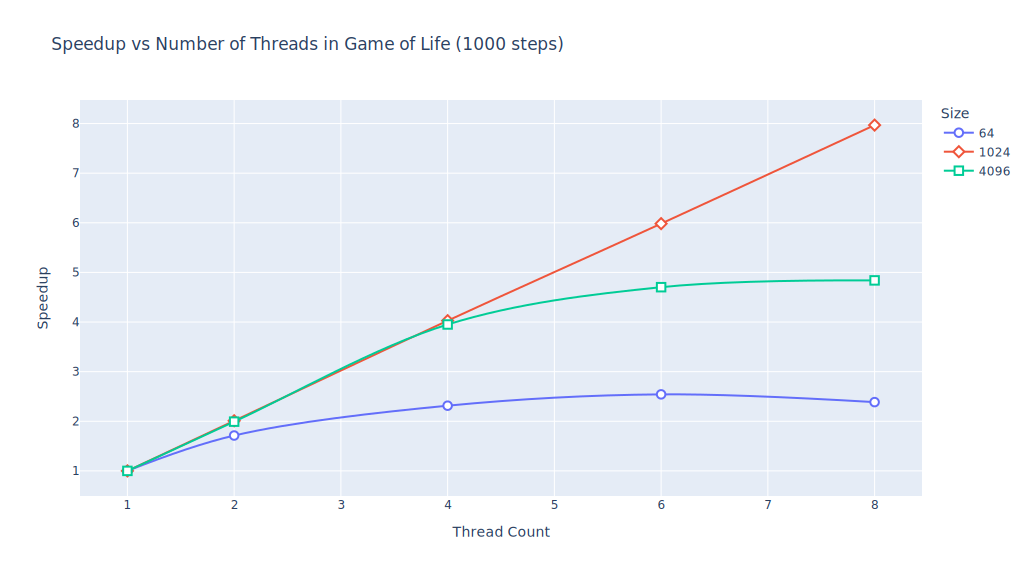
\includegraphics[width=\textwidth]{../a1/report/graphs/speedup_game_of_life.png} 
        \caption{Speedup of \eng{Game Of Life} for various game sizes.}
        \label{fig:speedup}
    \end{subfigure}
\end{figure}
\FloatBarrier

In Figure \ref{fig:stats}, three curves are shown—one for each \eng{Game of Life} simulation size—depicting runtime for various thread counts. Figure \ref{fig:speedup} shows three curves depicting the speedup for each simulation size.

\section{Interpretation of Results}

Both $64 \times 64$ and $4096 \times 4096$ do not scale.

For $64 \times 64$, execution is so fast that thread creation alone introduces enough overhead to prevent scaling. From 2 threads onward, scaling is non-ideal. There is speedup, just not as much as expected.

For $4096 \times 4096$, runtime is long enough that thread creation overhead is negligible. However, bus contention occurs because the data no longer fit in the \eng{cache}, so threads request data from main memory more frequently. The shared bus serializes part of the program, forcing some threads to wait for others to obtain their data. This emerges from 6 threads and above. Up to 4 threads, scaling is almost ideal.

In contrast, at $1024 \times 1024$ we observe ideal linear \eng{speedup} for all thread counts. Here, the parameters align so that there is no bus contention and the work distribution across threads is excellent.

\clearpage
\section{Appendix}

\begin{lstlisting}[caption={Parallelized Game Of Life}, style=CStyle, label={lst:parallelized-gol}]
...
for ( t = 0 ; t < T ; t++ ) {
    #pragma omp parallel for private(nbrs, i, j) shared(previous, current)
    for ( i = 1 ; i < N-1 ; i++ )
        for ( j = 1 ; j < N-1 ; j++ ) {
            nbrs = previous[i+1][j+1] + previous[i+1][j] + previous[i+1][j-1] \
                 + previous[i][j-1] + previous[i][j+1] \
                 + previous[i-1][j-1] + previous[i-1][j] + previous[i-1][j+1];
            if ( nbrs == 3 || ( previous[i][j]+nbrs ==3 ) )
                current[i][j]=1;
            else
                current[i][j]=0;
        }
        #ifdef OUTPUT
        print_to_pgm(current, N, t+1);
        #endif
        //Swap current array with previous array
        swap=current;
        current=previous;
        previous=swap;
}
... 
\end{lstlisting}

\begin{lstlisting}[caption={Bash Script to build Game Of Life}, language=bash, label={lst:make-gol}]
#!/bin/bash

## Give the Job a descriptive name
#PBS -N make_omp_gol

## Output and error files
#PBS -o make_omp_gol.out
#PBS -e make_omp_gol.err

## How many machines should we get? 
#PBS -l nodes=1:ppn=1

##How long should the job run for?
#PBS -l walltime=00:01:00

## Start 
## Run make in the src folder (modify properly)

module load openmp
cd /home/parallel/parlab30/a1
make
\end{lstlisting}

\begin{lstlisting}[caption={Makefile}, language=bash, label={lst:makefile}]
all: Game_Of_Life

Game_Of_Life: Game_Of_Life.c
	gcc -O3 -fopenmp -o Game_Of_Life Game_Of_Life.c

clean:
	rm Game_Of_Life
\end{lstlisting}

\clearpage
\begin{lstlisting}[caption={Bash Script to Gather Measurements}, language=bash, label={lst:run-gol}]
#!/bin/bash

## Give the Job a descriptive name
#PBS -N run_gol

## Output and error files
#PBS -o .run.out
#PBS -e .run.err

## How many machines should we get? 
#PBS -l nodes=1:ppn=8

##How long should the job run for?
#PBS -l walltime=00:10:00

## Start 
## Run make in the src folder (modify properly)

module load openmp
cd /home/parallel/parlab30/a1

threads=(1 2 4 6 8)
sizes=(64 1024 4096)
speed=1000

for thread in "${threads[@]}"
do
    export OMP_NUM_THREADS="$thread"
    for size in "${sizes[@]}"
    do
        ./Game_Of_Life "$size" "$speed"
    done
done
\end{lstlisting}

% ============================
% Exercise 2
% ============================
\clearpage
\part{Exercise 2}

\section{\eng{K-MEANS}}

\subsection{\eng{shared clusters}}

The code was parallelized by adding the appropriate \eng{OMP compiler directives} at the parallelizable points of the program (see \ref{lst:kmeans-shared-clusters}). The measurements are presented in Figure \ref{fig:kmeans-naive-shared-clusters}. It is observed that, in every case, regardless of thread count, the parallel version of the algorithm is slower than the serial version. This is because the attempted parallelization was naive. Specifically, all threads share the arrays with cluster data, which wastes a lot of compute time on synchronization. Notably, even for a single thread, the parallel version is slower. This is due to the use of atomic instructions for synchronization, which lock the bus and interfere with processor acceleration features. In the serial algorithm, atomic operations are absent because atomicity is inherent.

\begin{figure}[h]
    \centering
    \includegraphics[width=\textwidth]{a2/plots/kmeans_naive_time_speedup.png}
    \caption{Execution Time and \eng{Speedup} of \eng{Naive Kmeans Shared Clusters}}
    \label{fig:kmeans-naive-shared-clusters}
\end{figure}
\FloatBarrier

If the environment variable \eng{GOMP\_CPU\_AFFINITY} is set appropriately, threads remain pinned to a processor during their lifetime. This ensures they are not moved to another core and that they retain data locality.

\begin{figure}[h]
    \centering
    \includegraphics[width=\textwidth]{a2/plots/kmeans_naive_time_speedup_aff_on.png}
    \caption{\eng{Speedup} of \eng{Naive Kmeans Shared Clusters} with CPU Affinity on}
    \label{kmeans_naive_time_speedup_aff_on}
\end{figure}
\FloatBarrier

It appears to have little impact on runtime, which is expected, since the underlying issue was different and not related to thread migration across cores.

\subsection{\eng{copied clusters and reduce}}

\begin{figure}[h]
    \centering
    \includegraphics[width=\textwidth]{a2/plots/kmeans_copy_reduce_time_speedup.png}
    \caption{\eng{Speedup} of \eng{Kmeans Copy Reduce}}
    \label{kmeans_copy_reduce_time_speedup}
\end{figure}
\FloatBarrier

We observe much better scaling and nearly perfect linear \eng{speedup}. In this implementation, each thread has its own copy of the \eng{clusters}, and these are combined at the end of each iteration. As a result, there is no resource contention, greatly reducing runtime. There is only a small synchronization \eng{overhead} at the end of each iteration. Note that good performance is also helped by \eng{CPU\_AFFINITY}, which reduces thread migrations across processors and preserves data locality.

\begin{figure}[h]
    \centering
    \includegraphics[width=\textwidth]{a2/plots/kmeans_copy_reduce_time_speedup_false_sharing.png}
    \caption{\eng{Speedup} of \eng{Naive Kmeans Shared Clusters}}
    \label{fig:kmeans-naive-shared-clusters-false-sharing}
\end{figure}

Running \eng{getconf -a | grep CACHE} on \eng{scirouter} shows each cache level has \eng{cache line size} = 64 \eng{Bytes}. In configuration \eng{\{256, 1, 4, 10\}}, the center of each \eng{cluster} is a point represented by a \eng{double = 8 bytes}. This means one cache line fits two copies of the \eng{local newClusters} arrays. Consequently, data from each thread are not actually isolated; they end up on the same cache line, copies of that line are stored in caches of many cores, and the coherence protocol is triggered, even though there is no real data sharing. This causes bus traffic and significant delay.

One solution is to exploit Linux's \eng{first touch} policy (\ref{lst:kmeans-first-touch}).

\begin{figure}[h]
    \centering
    \includegraphics[width=\textwidth]{a2/plots/kmeans_copy_reduce_time_speedup_first_touch.png}
    \caption{\eng{Speedup} of \eng{Kmeans Copy Reduce First Touch}}
    \label{fig:kmeans_copy_reduce_time_speedup_first_touch}
\end{figure}

Another solution is to allocate more space than necessary per thread, effectively inserting zeros in the cache line and thus avoiding \eng{false sharing} (\ref{lst:kmeans-zero-padding}).

\begin{figure}[h]
    \centering
    \includegraphics[width=\textwidth]{a2/plots/kmeans_copy_reduce_time_speedup_zero_padding.png}
    \caption{\eng{Speedup} of \eng{Kmeans Copy Reduce Zero Padding}}
    \label{fig:kmeans_copy_reduce_time_speedup_zero_padding}
\end{figure}

Of course, both methods can be used simultaneously.

\begin{figure}[h]
    \centering
    \includegraphics[width=\textwidth]{a2/plots/kmeans_copy_reduce_time_speedup_both.png}
    \caption{\eng{Speedup} of \eng{Kmeans Copy Reduce Both}}
    \label{fig:kmeans_copy_reduce_time_speedup_both}
\end{figure}

Ultimately, the \eng{Zero Padding} method scales better.

\clearpage
\section{\eng{Floyd-Warshall}}

The recursive implementation \ref{lst:fw-rec} of the \eng{Floyd–Warshall} algorithm, while it initially improves runtime, does not scale satisfactorily. This is expected because the \eng{task graph} does not exhibit much parallelism. Of the eight recursive calls, only four are pairwise parallel, i.e., their data do not depend on one another. Therefore, we parallelize only one of the two \eng{tasks} for two total calls out of eight, and effectively only one \eng{extra thread} is used regardless of how many were created. Thus, going from 1 to 2 threads reduces runtime by about 25\% minus thread-creation overhead, since the 8 \eng{tasks} of the recursion complete in the time of \eng{6 tasks}. Beyond this point, extra threads do not further reduce runtime; they only add creation overhead.

\begin{figure}[h]
    \centering
    \begin{subfigure}{0.49\textwidth}
        \includegraphics[width=\textwidth]{a2/plots/fw_1024.png}
        \caption{\eng{Floyd Warshall} recursive 1024}
    \end{subfigure}
    \begin{subfigure}{0.49\textwidth}
        \includegraphics[width=\textwidth]{a2/plots/fw_2048.png}
        \caption{\eng{Floyd Warshall} recursive 2048}
    \end{subfigure}
    \begin{subfigure}{0.49\textwidth}
        \includegraphics[width=\textwidth]{a2/plots/fw_4096.png}
        \caption{\eng{Floyd Warshall} recursive 4096}
    \end{subfigure}
\end{figure}

The \eng{tiled} version \ref{lst:fw-tiled} exhibits more parallelism, which is reflected in the runtime plots: scaling is clearly satisfactory. Note that scaling degrades earlier for small sizes than for large ones. This relates to problem size versus the cost of spawning more \eng{threads}. Scaling “breaks” where thread-creation time exceeds the time saved by parallelization. The time saved by parallelization varies with problem size, while the time to create a given number of threads remains constant, leading to different breakpoints depending on problem size. Specifically, at 1024 the breakpoint is at 16 threads; at 2048, somewhere between 32–64 threads; and at 4096, at 64 threads and beyond.

\begin{figure}[h]
    \centering
    \begin{subfigure}{0.49\textwidth}
        \includegraphics[width=\textwidth]{a2/plots/fw_tiled_1024.png}
        \caption{\eng{Floyd Warshall tiled} 1024}
        \label{fig:fw_tiled_1024}
    \end{subfigure}
    \begin{subfigure}{0.49\textwidth}
        \includegraphics[width=\textwidth]{a2/plots/fw_tiled_2048.png}
        \caption{\eng{Floyd Warshall tiled} 2048}
        \label{fig:fw_tiled_2048}
    \end{subfigure}
    \begin{subfigure}{0.49\textwidth}
        \includegraphics[width=\textwidth]{a2/plots/fw_tiled_4096.png}
        \caption{\eng{Floyd Warshall tiled} 4096}
        \label{fig:fw_tiled_4096}
    \end{subfigure}
\end{figure}

\clearpage
\section{Appendix}

\begin{lstlisting}[caption={Naive Kmeans Shared Clusters}, style=CStyle, label={lst:kmeans-shared-clusters}]
...
#pragma omp parallel for private(i, j, index) shared(numObjs, delta, newClusterSize, newClusters)
for (i=0; i<numObjs; i++) {
    // find the array index of nearest cluster center 
    index = find_nearest_cluster(numClusters, numCoords, &objects[i*numCoords], clusters);

    // if membership changes, increase delta by 1 
    if (membership[i] != index)
        #pragma omp atomic
        delta += 1.0;

    // assign the membership to object i 
    membership[i] = index;

    // update new cluster centers : sum of objects located within 
    /*
     * TODO: protect update on shared "newClusterSize" array
     */
    #pragma omp atomic 
    newClusterSize[index]++;
    for (j=0; j<numCoords; j++)
        /*
         * TODO: protect update on shared "newClusters" array
         */
        #pragma omp atomic 
        newClusters[index*numCoords + j] += objects[i*numCoords + j];
}
// average the sum and replace old cluster centers with newClusters 
for (i=0; i<numClusters; i++) {
    if (newClusterSize[i] > 0) {
        for (j=0; j<numCoords; j++) {
            clusters[i*numCoords + j] = newClusters[i*numCoords + j] / newClusterSize[i];
        }
    }
}
... 
\end{lstlisting}

\begin{lstlisting}[caption={Kmeans First Touch}, style=CStyle, label={lst:kmeans-first-touch}]
...
#pragma omp parallel for private(k)
for (k=0; k<nthreads; k++)
{
        local_newClusterSize[k] = (typeof(*local_newClusterSize)) calloc(numClusters, sizeof(**local_newClusterSize));
        local_newClusters[k] = (typeof(*local_newClusters)) calloc(numClusters * numCoords, sizeof(**local_newClusters));
}
... 
\end{lstlisting}

\begin{lstlisting}[caption={Kmeans Zero Padding}, style=CStyle, label={lst:kmeans-zero-padding}]
...
#define CACHE_LINE_SIZE 64
#define PADDING_DOUBLE (CACHE_LINE_SIZE - sizeof(double))

// Each thread calculates new centers using a private space. After that, thread 0 does an array reduction on them.
int * local_newClusterSize[nthreads];  // [nthreads][numClusters] 
double * local_newClusters[nthreads];   // [nthreads][numClusters][numCoords]

for (k=0; k<nthreads; k++)
{
        local_newClusterSize[k] = (typeof(*local_newClusterSize)) calloc(numClusters, sizeof(**local_newClusterSize));
        local_newClusters[k] = (typeof(*local_newClusters)) calloc(numClusters * numCoords + numClusters * PADDING_DOUBLE, sizeof(**local_newClusters));
}
... 
\end{lstlisting}

\begin{lstlisting}[caption={FW Recursive}, style=CStyle, label={lst:fw-rec}]
...
else {  // This is called as FW_SR(A, A, A) so A, B, C are the same array.
    #pragma omp parallel
    {
        #pragma omp single
        {
            FW_SR(A,arow, acol,B,brow, bcol,C,crow, ccol, myN/2, bsize); // A00, B00, C00

            #pragma omp task
            FW_SR(A,arow, acol+myN/2,B,brow, bcol,C,crow, ccol+myN/2, myN/2, bsize); // A01, B00, C01
            #pragma omp task if(0)
            {
                    FW_SR(A,arow+myN/2, acol,B,brow+myN/2, bcol,C,crow, ccol, myN/2, bsize); // A10, B10, C00
            }
            #pragma omp taskwait

            FW_SR(A,arow+myN/2, acol+myN/2,B,brow+myN/2, bcol,C,crow, ccol+myN/2, myN/2, bsize); // A11, B10, C01


            FW_SR(A,arow+myN/2, acol+myN/2,B,brow+myN/2, bcol+myN/2,C,crow+myN/2, ccol+myN/2, myN/2, bsize); // A11, B11, C11

            #pragma omp task
            FW_SR(A,arow+myN/2, acol,B,brow+myN/2, bcol+myN/2,C,crow+myN/2, ccol, myN/2, bsize); // A10, B11, C10
            #pragma omp task if(0)
            {
                    FW_SR(A,arow, acol+myN/2,B,brow, bcol+myN/2,C,crow+myN/2, ccol+myN/2, myN/2, bsize); // A01, B01, C11
            }
            #pragma omp taskwait
            FW_SR(A,arow, acol,B,brow, bcol+myN/2,C,crow+myN/2, ccol, myN/2, bsize); // A00, B01, C10
        }
    }
}
...
\end{lstlisting}

\begin{lstlisting}[caption={FW Tiled}, style=CStyle, label={lst:fw-tiled}]
...
for(k=0;k<N;k+=B){
        FW(A,k,k,k,B); // top-left corner

        # pragma omp parallel for private(i)
        for(i=0; i<k; i+=B)
                FW(A,k,i,k,B);

        # pragma omp parallel for private(i)
        for(i=k+B; i<N; i+=B)
                FW(A,k,i,k,B);

        # pragma omp parallel for private(j)
        for(j=0; j<k; j+=B)
                FW(A,k,k,j,B);

        # pragma omp parallel for private(j)
        for(j=k+B; j<N; j+=B)
                FW(A,k,k,j,B);

        # pragma omp parallel for private(i, j)
        for(i=0; i<k; i+=B)
                for(j=0; j<k; j+=B)
                        FW(A,k,i,j,B);

        # pragma omp parallel for private(i, j)
        for(i=0; i<k; i+=B)
                for(j=k+B; j<N; j+=B)
                        FW(A,k,i,j,B);

        # pragma omp parallel for private(i, j)
        for(i=k+B; i<N; i+=B)
                for(j=0; j<k; j+=B)
                        FW(A,k,i,j,B);

        # pragma omp parallel for private(i, j)
        for(i=k+B; i<N; i+=B)
                for(j=k+B; j<N; j+=B)
                        FW(A,k,i,j,B);
}
...
\end{lstlisting}

% ============================
% Exercise 3
% ============================
\clearpage
\part{Exercise 3}

\section{\eng{K-MEANS}}

\subsection{Mutual Exclusion — Locks}

Qualitatively, all implementations—except \eng{array lock} and \eng{clh lock}—show the same behavior: they maintain speedup up to 4 threads at best and exhibit large slowdowns for 8 threads and above. Their differences are mainly in absolute timings. This behavior stems from locks being mainly suitable for sporadic accesses to shared data to maintain correctness. Here, all threads simultaneously request access to shared data throughout execution, leading to congestion and, effectively, serialization.

Specifically, \eng{pthread mutex lock} (Fig.~\ref{fig:mutex}) performs worse already at 8 threads and shows a sharp runtime increase for more threads, reaching up to 4 seconds in the worst case. \eng{pthread spin lock} (Fig.~\ref{fig:spin}) behaves similarly but is even slower beyond 16 threads because \eng{mutex} locks put threads to sleep (freeing resources), whereas \eng{spin} locks busy-wait and consume compute resources.

This thread count is not arbitrary: the system has 4 sockets with 4 cores each, supporting up to 2 hardware threads per core—i.e., up to 32 hardware threads in the best case—assuming varied workloads (not true here), so contention is severe.

\eng{test and set} (Fig.~\ref{fig:tas}) and \eng{test and test and set} (Fig.~\ref{fig:ttas}) locks show similar behavior and are even slower, as they are hardware-level primitives typically suitable for short critical sections. Our application locks relatively large critical sections. \eng{TTAS} is faster than \eng{TAS} because \eng{TAS} triggers coherence traffic (\eng{bus read x}) on every attempt, while \eng{TTAS} first reads (\eng{bus read}) and only escalates if needed.

\eng{array lock} (Fig.~\ref{fig:array}) and \eng{clh lock} (Fig.~\ref{fig:clh}) perform much better. They allow speedup up to 8 threads and remain faster than other locks even when parallel execution becomes slower than serial ($>16$ threads). They coordinate across multiple locks at different memory locations rather than contending on a single lock. In \eng{array lock}, a boolean array of length equal to the number of threads assigns each thread a lock position; a thread proceeds only when its position is \eng{true}, then hands off to the next. \eng{CLH} improves upon \eng{array lock} with less bus contention and memory usage.

\begin{figure}[ht]
    \centering
    \begin{subfigure}{0.45\textwidth}
        \includegraphics[width=\textwidth]{a3/plots/nosync_lock.png}
        \caption{\eng{no sync lock}}
        \label{fig:nosync}
    \end{subfigure}
    \begin{subfigure}{0.45\textwidth}
        \includegraphics[width=\textwidth]{a3/plots/pthread_mutex_lock.png}
        \caption{\eng{pthread mutex lock}}
        \label{fig:mutex}
    \end{subfigure}
    \vspace{1em}
    \begin{subfigure}{0.45\textwidth}
        \includegraphics[width=\textwidth]{a3/plots/pthread_spin_lock.png}
        \caption{\eng{pthread spin lock}}
        \label{fig:spin}
    \end{subfigure}
    \begin{subfigure}{0.45\textwidth}
        \includegraphics[width=\textwidth]{a3/plots/tas_lock.png}
        \caption{\eng{test and set lock}}
        \label{fig:tas}
    \end{subfigure}
\end{figure}

\begin{figure}
    \centering
    \ContinuedFloat
    \begin{subfigure}{0.45\textwidth}
        \includegraphics[width=\textwidth]{a3/plots/ttas_lock.png}
        \caption{\eng{test and test and set lock}}
        \label{fig:ttas}
    \end{subfigure}
    \begin{subfigure}{0.45\textwidth}
        \includegraphics[width=\textwidth]{a3/plots/array_lock.png}
        \caption{\eng{array lock}}
        \label{fig:array}
    \end{subfigure}
    \vspace{1em}
    \begin{subfigure}{0.6\textwidth}
        \includegraphics[width=\textwidth]{a3/plots/clh_lock.png}
        \caption{\eng{clh lock}}
        \label{fig:clh}
    \end{subfigure}
\end{figure}
\FloatBarrier

\subsection{Concurrent Data Structures}

The \eng{coarse-grain locking} implementation (Fig.~\ref{fig:cgl}) shows decreasing throughput as threads increase, as the entire structure is locked for any operation. Even with 100\% lookups, performance drops. The effect is worse when operations beyond search are involved (locks held longer). On longer lists the effect is less pronounced, since search is already time-consuming.

The \eng{fine-grain locking} implementation (Fig.~\ref{fig:fgl}) has worse single-thread throughput than coarse (lock overhead), but it does not drop further as threads increase; it remains almost flat.

The \eng{optimistic} implementation (Fig.~\ref{fig:opt}) scales throughput better by locking only the node that needs modification, eliminating repeated lock/unlock overhead on every node. At 128 threads, a drop appears—likely many threads attempt many operations concurrently and impede each other.

The \eng{lazy locking} implementation (Fig.~\ref{fig:lazy}) scales well, especially for read-only workloads, because reads do not lock and traverse the list without locks. Other cases also improve over optimistic because \eng{validate} does not traverse the entire list. Scaling “stalls” near 128 threads, likely due to the limitations of hyperthreading when many hardware threads contend for identical resources.

The \eng{non-blocking} implementation (Fig.~\ref{fig:nb}) scales better than lazy except for read-only cases, likely due to higher structural overhead but more scalable add/remove (no blocking). Up to 16 threads lazy is more efficient; at 32–64 they are similar; at 128 non-blocking is faster.

\begin{figure}[ht]
    \centering
    \begin{subfigure}{0.45\textwidth}
        \includegraphics[width=\textwidth]{a3/plots/cgl.png}
        \caption{\eng{coarse-grain locking}}
        \label{fig:cgl}
    \end{subfigure}
    \begin{subfigure}{0.45\textwidth}
        \includegraphics[width=\textwidth]{a3/plots/fgl.png}
        \caption{\eng{fine-grain locking}}
        \label{fig:fgl}
    \end{subfigure}
    \vspace{1em}
    \begin{subfigure}{0.45\textwidth}
        \includegraphics[width=\textwidth]{a3/plots/opt.png}
        \caption{\eng{optimistic locking}}
        \label{fig:opt}
    \end{subfigure}
    \begin{subfigure}{0.45\textwidth}
        \includegraphics[width=\textwidth]{a3/plots/lazy.png}
        \caption{\eng{lazy locking}}
        \label{fig:lazy}
    \end{subfigure}
\end{figure}

\begin{figure}
    \centering
    \ContinuedFloat
    \begin{subfigure}{0.8\textwidth}
        \includegraphics[width=\textwidth]{a3/plots/nb.png}
        \caption{\eng{non-blocking locking}}
        \label{fig:nb}
    \end{subfigure}
\end{figure}
\clearpage

The comparison of implementations is also summarized very briefly by the table below:

\begin{figure}
    \centering
    \ContinuedFloat
    \begin{subfigure}{0.8\textwidth}
        \includegraphics[width=\textwidth]{a3/plots/comparing_screenshots.png}
        \caption{Source: course notes}
    \end{subfigure}
\end{figure}

% ============================
% Exercise 4
% ============================
\clearpage
\part{Exercise 4}

\section{\eng{Naive}}
\begin{figure}[h]\centering
        \includegraphics[width=0.7\textwidth]{a4/plots/kmeans_seq_vs_naive.png}
        \caption{Execution time}
\end{figure}\FloatBarrier

The parallel implementation is faster than the serial baseline. Offloading the heavy compute to the \eng{GPU} yields almost an order-of-magnitude speedup (about $\times 10$). Regarding \eng{block} size, performance is relatively stable. Generally, performance versus \eng{block size} is influenced via \eng{occupancy}. Thus either occupancy is constant and independent of \eng{block size} (possibly 100\%) or total time is dominated by CPU–GPU communication and the GPU executes the compute portion quickly. On our GPU:
\begin{equation}
\eng{block\_size\_for\_max\_occupancy} \ge 
\frac{\eng{number\_of\_max\_blocks}}{\eng{total\_threads}} = \frac{2048}{32} = 64
\end{equation}
This is reflected in the plots: a slight speedup for \eng{block size} $\ge 64$ threads.

\clearpage
\section{\eng{Transpose}}
\begin{figure}[h]\centering
        \includegraphics[width=0.7\textwidth]{../a4/plots/kmeans_seq_vs_naive_vs_trans.png}
        \caption{Execution time}
\end{figure}\FloatBarrier

The \eng{transpose} implementation again outperforms \eng{naive} yet remains relatively independent of \eng{block size}. This likely stems from better memory coalescing with \eng{transpose}: data needed by each \eng{warp} are contiguous—something that may not hold in the \eng{naive} approach. \eng{Transpose} changes how the GPU accesses data, not algorithmic complexity.

\section{\eng{Shared}}
\begin{figure}[h]\centering
        \includegraphics[width=0.7\textwidth]{../a4/plots/kmeans_seq_vs_naive_vs_trans_vs_shmem.png}
        \caption{Execution time}
\end{figure}

The \eng{shared memory} implementation provides another performance step beyond \eng{transpose}, and again appears fairly independent of \eng{(thread) block size}. Overall runtime is dominated by data movement; \eng{shared memory} mitigates this by allowing threads to update on-chip shared memory. Hence, execution time is not strongly affected by \eng{block size}.

\begin{figure}[h]\centering
    \begin{subfigure}{0.45\textwidth}
        \includegraphics[width=\textwidth]{../a4/plots/execution_time.png}
        \caption{Execution time} 
        \label{fig:speedup_kmeans_n-t-s}
    \end{subfigure}
    \begin{subfigure}{0.45\textwidth}
        \includegraphics[width=\textwidth]{../a4/plots/speedup.png}
        \caption{\eng{speedup}}
    \end{subfigure}
    \vspace{1em}
    \begin{subfigure}{0.6\textwidth}
        \includegraphics[width=\textwidth]{../a4/plots/kmeans_execution_time_vs_serial.png}
        \caption{Execution time compared to \eng{serial}}
        \label{fig:timekm-ser}
    \end{subfigure}
\end{figure}
\FloatBarrier

\clearpage
\section{\eng{Bottleneck Analysis}}

\subsection{\eng{2 Coordinates}}

For two dimensions (see Fig.~\ref{fig:naive_pbs2}), CPU time dominates in every case and is unaffected by \eng{block size} or method (\eng{naive}, \eng{transpose}, \eng{shared}), since the CPU-side work is unchanged. GPU$\rightarrow$CPU transfer time is also stable across methods and block sizes; CPU$\rightarrow$GPU transfer is about three orders of magnitude smaller and nearly constant (variation $<5\%$), so a log scale adds little value.

GPU compute time decreases from \eng{naive} to \eng{transpose} (better coalescing). \eng{Shared} also improves memory access vs \eng{naive} but not much over \eng{transpose} in 2D because the huge number of objects introduces many race conditions. With 16D, \eng{shared} will show clearer gains.

Regarding \eng{block size}, in 2D all times remain relatively stable regardless of method, likely because \eng{block size} is much larger than the maximum parallelism the system can exploit. Objects vastly outnumber the maximum block sizes, so rounding to a larger block size does not matter.

The GPU provides 32 FP64 units per SM; since the kernel is FP64-heavy, not all thread demands can be satisfied simultaneously.

\begin{figure}[h]
    \centering
    \begin{subfigure}{0.65\textwidth}
        \includegraphics[width=\textwidth]{../a4/plots/PBS_naive_kmeans_bottleneck.png}
        \caption{\eng{naive} execution time versus \eng{block size}}
        \label{fig:naive_pbs2}
    \end{subfigure}
    \begin{subfigure}{0.65\textwidth}
        \includegraphics[width=\textwidth]{../a4/plots/PBS_transpose_kmeans_bottleneck.png}
        \caption{\eng{transpose} execution time versus \eng{block size}}
        \label{fig:transpose_pbs2}
    \end{subfigure}
    \begin{subfigure}{0.65\textwidth}
        \includegraphics[width=\textwidth]{../a4/plots/PBS_shared_kmeans_bottleneck.png}
        \caption{\eng{shared} execution time versus \eng{block size}}
        \label{fig:shared_pbs2}
    \end{subfigure}
    \caption{\eng{configuration with coordinate dim = 2}}
\end{figure}
\FloatBarrier

\clearpage
\subsection{\eng{16 coordinates}}

Although the total data volume remains constant, CPU compute time decreases. The relevant code is shown for clarity:

\begin{lstlisting}[style=CStyle]
/* CPU part: Update cluster centers*/  		
for (i=0; i<numObjs; i++) {
    /* find the array index of nestest cluster center */
    index = membership[i];
    
    /* update new cluster centers : sum of objects located within */
    newClusterSize[index]++;
    for (j=0; j<numCoords; j++)
        newClusters[j][index] += objects[i*numCoords + j];
}
/* average the sum and replace old cluster centers with newClusters */
for (i=0; i<numClusters; i++) {
    for (j=0; j<numCoords; j++) {
        if (newClusterSize[i] > 0)
            clusters[i*numCoords + j] = newClusters[i][j] / newClusterSize[i];
        newClusters[j][i] = 0.0;   /* set back to 0 */
    }
    newClusterSize[i] = 0;   /* set back to 0 */
}
\end{lstlisting}

The number of objects is reduced by a factor of eight. Therefore, the first double loop executes $16777216 * 3 - 2097152 * 3 = 44{,}040{,}192$ fewer instructions (notably fewer accesses to \eng{membership} and \eng{newClusterSize}). The second double loop executes $16 * 16 - 16 * 2 = 224$ more instructions—negligible compared to the large reduction in the first loop.

GPU$\rightarrow$CPU transfer time is also divided by eight, meaning that increased parallelism enabled by more dimensions (independent per dimension) is fully reflected in transfers (time drops from $\sim0.16$ to $\sim0.02$). Transfer cost scales per object; e.g., the \eng{membership} buffer has size equal to the number of objects.

\begin{figure}[h]
    \centering
    \begin{subfigure}{0.65\textwidth}
        \includegraphics[width=\textwidth]{../a4/plots/PBS_naive_kmeans_bottleneck_16.png}
        \caption{\eng{naive} execution time versus \eng{block size}}
        \label{fig:naive_pbs16}
    \end{subfigure}
    \begin{subfigure}{0.65\textwidth}
        \includegraphics[width=\textwidth]{../a4/plots/PBS_transpose_kmeans_bottleneck_16.png}
        \caption{\eng{transpose} execution time versus \eng{block size}}
        \label{fig:transpose_pbs16}
    \end{subfigure}
    \vspace{1em}
    \begin{subfigure}{0.65\textwidth}
        \includegraphics[width=\textwidth]{../a4/plots/PBS_shared_kmeans_bottleneck_16.png}
        \caption{\eng{shared} execution time versus \eng{block size}}
        \label{fig:shared_pbs16}
    \end{subfigure}
    \caption{\eng{configuration with coordinate dim = 16}}
\end{figure}
\FloatBarrier

\clearpage
\section{\eng{Bonus: Full Offload (All-GPU) version}}

For the “ALL GPU” version, with more coordinates and the same total data volume (thus eight times fewer objects), execution is faster because coordination costs for cluster sizes and centroid updates are smaller: one-eighth the objects compete for eight times the per-dimension resources.

\eng{update\_centroids} was implemented partly in \eng{find\_nearest\_cluster}: immediately after finding the nearest cluster, atomic updates effectively perform \eng{reduce(+)} of members and cluster sizes. Then \eng{update\_centroids} assigns each thread a cluster and a dimension and divides by the cluster size to compute the mean (see \ref{lst:gpu-kmeans-allgpu}).

As noted, the GPU provides 32 FP64 units per SM; not all thread demands can be satisfied simultaneously. In 2D, each thread uses resources for less time than in 16D, so warp schedulers can issue other warps more often. With 4 warp schedulers per SM, any improvement will be visible up to 128 threads per block. Beyond that, contention is very high.

The 16D experiment appears to suffer from \eng{warp blockage}. An SM cannot evict a block and replace it with another until the last warp completes. With large blocks (many warps), SM resources are more likely to be exhausted, delaying some warps and thus the entire block. Also, with larger blocks at fixed problem size, there are fewer blocks overall—fewer choices for scheduling can also cause delays. This is visible up to 64 threads per block. The behavior at other block sizes likely relates to moving \eng{update\_centroids} to the GPU.

\begin{figure}[h]
    \centering
    \begin{subfigure}{0.45\textwidth}
        \includegraphics[width=\textwidth]{a4/plots/all_gpu_2.png}
        \caption{\eng{all GPU} execution time, 2 coordinates}
        \label{fig:all-gpu-2}
    \end{subfigure}
    \begin{subfigure}{0.45\textwidth}
        \includegraphics[width=\textwidth]{a4/plots/all_gpu_16.png}
        \caption{\eng{all GPU} execution time, 16 coordinates}
        \label{fig:all-gpu-16}
    \end{subfigure}
    \vspace{1em}
    \begin{subfigure}{0.45\textwidth}
        \includegraphics[width=\textwidth]{a4/plots/all_gpu_2_speedup.png}
        \caption{\eng{All GPU Speedup}, 2 coordinates}
        \label{fig:all-gpu-2-speedup}
    \end{subfigure}
    \begin{subfigure}{0.45\textwidth}
        \includegraphics[width=\textwidth]{a4/plots/all_gpu_16_speedup.png}
        \caption{\eng{All GPU Speedup}, 16 coordinates}
        \label{fig:all-gpu-16-speedup}
    \end{subfigure}
\end{figure}
\FloatBarrier

\eng{update\_centroids} is well-suited to the GPU because it can be implemented with perfect parallelism. From the bottlenecks, the worst time is \eng{CPU Total} (CPU compute time). The all-GPU approach eliminates a large portion of this time and thus mitigates the bottleneck.

The second configuration has more dimensions; the performance difference arises because it performs eight times more per-object coordinate work on the GPU but with far fewer objects and better parallel efficiency.

\clearpage
\section{Appendix} % code excerpts
\textbf{\eng{Skip} the code below: \hyperref[chapter_5]{\textit{\eng{Skip Code}}}}
\lstinputlisting[caption={Kmeans GPU Naive}, style=CStyle, label={lst:gpu-kmeans-naive}]{latex_cuda_naive.cu}
\clearpage
\lstinputlisting[caption={Kmeans GPU Transpose}, style=CStyle, label={lst:gpu-kmeans-transpose}]{latex_cuda_transpose.cu}
\clearpage
\lstinputlisting[caption={Kmeans GPU Shared}, style=CStyle, label={lst:gpu-kmeans-shared}]{latex_cuda_shared.cu}
\clearpage
\lstinputlisting[caption={Kmeans All GPU}, style=CStyle, label={lst:gpu-kmeans-allgpu}]{latex_cuda_allgpu.cu}

% ============================
% Exercise 5
% ============================
\clearpage
\part{Exercise 5}
\label{chapter_5}

\section{\eng{K-MEANS}}

\subsection{\eng{MPI} Implementation}

From the plots, scaling is highly satisfactory, achieving nearly ideal \eng{speedup}.

\begin{figure}[h]
    \centering
    \begin{subfigure}{0.45\textwidth}
        \includegraphics[width=\textwidth]{a5/plots/kmeans_mpi.png}
        \caption{Execution time, comparison (excluding serial)}
    \end{subfigure}
    \begin{subfigure}{0.45\textwidth}
        \includegraphics[width=\textwidth]{a5/plots/kmeans_mpi_log.png}
        \caption{Execution time (log scale)}
    \end{subfigure}
    \vspace{1em}
    \begin{subfigure}{0.45\textwidth}
        \includegraphics[width=\textwidth]{a5/plots/kmeans_mpi_speedup.png}
        \caption{\eng{Speedup}}
    \end{subfigure}
    \begin{subfigure}{0.45\textwidth}
        \includegraphics[width=\textwidth]{a5/plots/kmeans_mpi_speedup_log.png}
        \caption{\eng{Speedup} (log scale)}
        \label{fig:kmeans-mpi-speedup}
    \end{subfigure}
\end{figure}
\FloatBarrier

\subsection{\eng{BONUS} Question: Comparison with \eng{OpenMP}}

Ignoring specific numeric values, the \eng{MPI} implementation (distributed memory model) scales better and does not show a tendency to degrade at higher process counts and data sizes, unlike the \eng{OpenMP} version. See, e.g., \ref{fig:kmeans_copy_reduce_time_speedup_zero_padding} vs \ref{fig:kmeans-mpi-speedup}.

\section{2D Heat Diffusion}

\subsection{Measurements with Convergence Check}

Figure \ref{fig:jacobi_conv_check} shows output from the parallel \eng{Jacobi} algorithm on a $1024 \times 1024$ grid with 64 processes. Most time is spent on inter-process communication. This is mainly due to the convergence check, which each process performs independently on its subgrid, and the use of \eng{MPI\_Allreduce} to combine results before proceeding.

We also note that the required iterations to converge are on the order of a million and that the temperature at the grid center is non-zero.

\begin{figure}[h]
    \small\verbatiminput{run_conv_check.out}
    \caption{Output Data \eng{Jacobi} $1024 \times 1024$}
    \label{fig:jacobi_conv_check}
\end{figure}
\FloatBarrier

\subsection{Measurements without Convergence Check}

Here (Fig.~\ref{fig:jacobi_no_conv_check}) the center temperature is zero, implying the algorithm likely did not converge and execution stopped early. This is expected: as noted earlier, convergence requires on the order of a million iterations, whereas here the limit is only 256 iterations.

\begin{figure}[h]
    \small\verbatiminput{run_no_conv_check.out}
    \caption{Output Data \eng{Jacobi} for various grid sizes.}
    \label{fig:jacobi_no_conv_check}
\end{figure}
\FloatBarrier

For the $2048 \times 2048$ grid, the total runtime scales satisfactorily and compute time scales very well, while communication time remains roughly constant (see \ref{fig:jacobi2048speedup}). Notably, at 64 threads the time is more than halved compared to 32 threads (\ref{fig:jacobi2048time}). This may be because the small grid fits well across processor caches. Beyond compute time, the rest (overhead, setup, inter-process communication) is relatively stable due to the smaller data volume.

For $4096 \times 4096$, compute time scales perfectly up to 8 processes (Fig.~\ref{fig:jacobi4096speedup}), and continues to scale (though non-ideally) up to 64 processes. Non-ideal scaling likely relates to cache capacity being insufficient for the larger problem. This also appears in the rising communication cost with more processes (\ref{fig:jacobi4096time}), since more processes imply higher communication costs when data no longer fit in cache.

Similarly, for $6144 \times 6144$, the hardware/setup does not favor this grid size; increasing process count makes communication significantly more difficult and costly.

Although behaviors for $4096^2$ and $6144^2$ look similar, the absolute communication time does scale up, from about half a second at the smallest to nearly six seconds at the largest problem.

\begin{figure}[ht]
    \centering
    \begin{subfigure}{0.45\textwidth}
        \includegraphics[width=\textwidth]{a5/plots/speedup-jacobi-small.png}
        \caption{\eng{speedup} $2048 \times 2048$}
        \label{fig:jacobi2048speedup}
    \end{subfigure}
    \begin{subfigure}{0.45\textwidth}
        \includegraphics[width=\textwidth]{a5/plots/speedup-jacobi-medium.png}
        \caption{\eng{speedup} $4096 \times 4096$}
        \label{fig:jacobi4096speedup}
    \end{subfigure}
    \vspace{1em}
    \begin{subfigure}{0.6\textwidth}
        \includegraphics[width=\textwidth]{a5/plots/speedup-jacobi-large.png}
        \caption{\eng{speedup} $6144 \times 6144$}
        \label{fig:jacobi6144speedup}
    \end{subfigure}
\end{figure}
\FloatBarrier

\begin{figure}[ht]
    \centering
    \begin{subfigure}{0.45\textwidth}
        \includegraphics[width=\textwidth]{a5/plots/bar-chart-Jacobi-small.png}
        \caption{Runtime breakdown $2048 \times 2048$}
        \label{fig:jacobi2048time}
    \end{subfigure}
    \begin{subfigure}{0.45\textwidth}
        \includegraphics[width=\textwidth]{a5/plots/bar-chart-Jacobi-medium.png}
        \caption{Runtime breakdown $4096 \times 4096$}
        \label{fig:jacobi4096time}
    \end{subfigure}
    \vspace{1em}
    \begin{subfigure}{0.6\textwidth}
        \includegraphics[width=\textwidth]{a5/plots/bar-chart-Jacobi-large.png}
        \caption{Runtime breakdown $6144 \times 6144$}
        \label{fig:jacobi6144time}
    \end{subfigure}
\end{figure}
\FloatBarrier

\clearpage
\section{Appendix} % code excerpts
\begin{lstlisting}[caption={Kmeans MPI}, style=CStyle, label={lst:mpi-kmeans}]
...
do {
    // before each loop, set cluster data to 0
    for (i=0; i<numClusters; i++) {
        for (j=0; j<numCoords; j++)
            rank_newClusters[i*numCoords + j] = 0.0;
        rank_newClusterSize[i] = 0;
    }
    rank_delta = 0.0;
    for (i=0; i<numObjs; i++) {
        // find the array index of nearest cluster center 
        index=find_nearest_cluster(numClusters,numCoords,&objects[i*numCoords],clusters);
        // if membership changes, increase rank_delta by 1 
        if (membership[i] != index)
            rank_delta += 1.0;
        // assign the membership to object i 
        membership[i] = index;
        // update new cluster centers : sum of objects located within
        rank_newClusterSize[index]++;
        for (j=0; j<numCoords; j++)
            rank_newClusters[index*numCoords + j] += objects[i*numCoords + j]; 
    }
    /*
     * TODO: Perform reduction of cluster data (rank_newClusters, rank_newClusterSize) from local arrays to shared.
     */
    MPI_Allreduce(rank_newClusters, newClusters, numClusters*numCoords, MPI_DOUBLE, MPI_SUM, MPI_COMM_WORLD);
    MPI_Allreduce(rank_newClusterSize, newClusterSize, numClusters, MPI_INT, MPI_SUM, MPI_COMM_WORLD);
    // average the sum and replace old cluster centers with newClusters
    for (i=0; i<numClusters; i++) {
        if (newClusterSize[i] > 0) {
            for (j=0; j<numCoords; j++) {
                clusters[i*numCoords + j] = newClusters[i*numCoords + j] / newClusterSize[i];
            }
        }
    }
    /*  
     * TODO: Perform reduction from rank_delta variable to delta variable, that will be used for convergence check.
     */
    MPI_Allreduce(&rank_delta, &delta, 1, MPI_DOUBLE, MPI_SUM, MPI_COMM_WORLD);

    // Get fraction of objects whose membership changed during this loop. This is used as a convergence criterion.
    delta /= numObjs;
    loop++;
} while (delta > threshold && loop < loop_threshold);
...
\end{lstlisting}

\begin{lstlisting}[caption={Jacobi MPI setup}, style=CStyle, label={lst:mpi-jacobi-setup}]
...
//----Ensure that u_current and u_previous are both initialized----//
init2d(u_current,local[0]+2,local[1]+2);
init2d(u_previous,local[0]+2,local[1]+2);
MPI_Scatterv(&(U[0][0]), scattercounts, scatteroffset, global_block, &(u_previous[1][1]), 1, local_block, 0, MPI_COMM_WORLD);
MPI_Scatterv(&(U[0][0]), scattercounts, scatteroffset, global_block, &(u_current[1][1]),  1, local_block, 0, MPI_COMM_WORLD);

if (rank==0) free2d(U);
MPI_Datatype row;
MPI_Type_contiguous(local[1], MPI_DOUBLE, &dummy);
MPI_Type_create_resized(dummy, 0, sizeof(double), &row);
MPI_Type_commit(&row);
MPI_Datatype column;
MPI_Type_vector(local[0], 1, local[1]+2, MPI_DOUBLE, &dummy);
MPI_Type_create_resized(dummy, 0, sizeof(double), &column);
MPI_Type_commit(&column);

//----Find the 4 neighbors with which a process exchanges messages----//
int north, south, east, west;

// the processes "in the middle" of the grid have 4 neighbors
// the processes on the edges have 3 neighbors
// the processes on the corners have 2 neighbors

MPI_Cart_shift(CART_COMM, 0, 1, &north, &south);
MPI_Cart_shift(CART_COMM, 1, 1, &west, &east);
...
\end{lstlisting}

\begin{lstlisting}[caption={Jacobi MPI ranges}, style=CStyle, label={lst:mpi-jacobi-ranges}]
...
//---Define the iteration ranges per process-----//
int i_min,i_max,j_min,j_max;
/*Three types of ranges:
-internal processes
-boundary processes
-boundary processes and padded global array
*/
// these are the ranges that will be used later for the double for loop
i_min = (north == MPI_PROC_NULL) ? 2 : 1;
j_min = (west == MPI_PROC_NULL) ? 2 : 1;
i_max = (south == MPI_PROC_NULL) ? local[0] - (global_padded[0] - global[0] + 1): local[0];
j_max = (east == MPI_PROC_NULL) ? local[1]- (global_padded[1] - global[1] + 1): local[1];
// because of the ghost cells, a 'normal' 'internal' process would start from its
// first row and column and end just before its last row and column
// if the process is on some edge, then the boundaries are shifted by one row (+) or column (-)
...
\end{lstlisting}

\begin{lstlisting}[caption={Jacobi MPI core}, style=CStyle, label={lst:mpi-jacobi-core}]
//----Computational core----//   
gettimeofday(&tts, NULL);
#ifdef TEST_CONV
for (t=0;t<T && !global_converged;t++) {
#endif
#ifndef TEST_CONV
#undef T
#define T 256
for (t=0;t<T;t++) {
#endif
    swap = u_previous;
    u_previous = u_current;
    u_current = swap;
    /*Compute and Communicate*/
    int count = 0;
    MPI_Request req[8];
    MPI_Status stat[8];
    gettimeofday(&tms,NULL);
    if (north != MPI_PROC_NULL)
    {
        MPI_Isend(&u_previous[1][1], 1, row, north, 0, MPI_COMM_WORLD, &req[count++]);
        MPI_Irecv(&u_previous[0][1], 1, row, north, 0, MPI_COMM_WORLD, &req[count++]);
    }
    if (south != MPI_PROC_NULL)
    {
        MPI_Isend(&u_previous[local[0]][1], 1, row,south, 0, MPI_COMM_WORLD, &req[count++]);
        MPI_Irecv(&u_previous[local[0]+1][1],1,row,south, 0, MPI_COMM_WORLD, &req[count++]);
    }
    if (east != MPI_PROC_NULL)
    {
        MPI_Isend(&u_previous[1][local[1]], 1,column,east,0,MPI_COMM_WORLD, &req[count++]);
        MPI_Irecv(&u_previous[1][local[1]+1],1,column,east,0,MPI_COMM_WORLD, &req[count++]);
    }
    if (west != MPI_PROC_NULL)
    {
        MPI_Isend(&u_previous[1][1], 1, column, west, 0, MPI_COMM_WORLD, &req[count++]);
        MPI_Irecv(&u_previous[1][0], 1, column, west, 0, MPI_COMM_WORLD, &req[count++]);
    }
    // Isend / Irecv do not block.
    MPI_Waitall(count, req, stat);
    gettimeofday(&tmf,NULL);
    tmsg += (tmf.tv_sec-tms.tv_sec)+(tmf.tv_usec-tms.tv_usec)*0.000001;
    gettimeofday(&tcs,NULL);
    for (i = i_min; i <= i_max; i++) {
        for (j = j_min; j <= j_max; j++) {
            u_current[i][j] = 0.25 * (u_previous[i-1][j] + u_previous[i+1][j]
                                   +  u_previous[i][j-1] + u_previous[i][j+1]);
        }
    }
    gettimeofday(&tcf,NULL);
    tcomp += (tcf.tv_sec-tcs.tv_sec)+(tcf.tv_usec-tcs.tv_usec)*0.000001;
    /*Add appropriate timers for computation*/
#ifdef TEST_CONV
    if (t%C==0) {
    /*Test convergence*/
        converged = converge(u_current, u_previous, i_min, i_max, j_min, j_max);
        MPI_Allreduce(&converged, &global_converged, 1, MPI_INT, MPI_MIN, MPI_COMM_WORLD);
    }
#endif
}
\end{lstlisting}

\end{document}
